\section[Propriétés de symétrie]{Propriétés de symétrie du champ électromagnétique}

    \subsection{Principe de Curie}

        Énoncé en 1905 par Pierre Curie :
        \begin{quote}[P. Curie, 1905]
            Les effets on au moins les symétries (et invariances) des causes.
        \end{quote}

    \subsection{Plans de symétrie (PS) ou d'antisymétrie (PAS) pour une distribution de charges et de courants}

        $(\pi)$ est un plan de symétrie pour une distribution de charges et de courants $\mathcal{D}$ si 
        \begin{equation}
            \rho(\pi(M),t)=\rho(M,t),\qquad \vec{j}(\pi(M),t)=S_{\pi}(\vec{j}(M,t)),
        \end{equation}
        où $\pi(M)$ désigne le symétrique du point $M$ et $S_{\pi}$ désigne l'application symétrie liée au plan $(\pi)$.

        C'est un plan d'anti-symétrie si
        \begin{equation}
            \rho(\pi(M),t)=-\rho(M,t),\qquad \vec{j}(\pi(M),t)=-S_{\pi}(\vec{j}(M,t)).
        \end{equation}

        \begin{example}[Solénoïde fini]
            Un solénoïde (enroulement jointif) contenant $N$ spires possède un PS et un PAS, voir la Figure~\ref{fig:plan_symetrie_solenoide_fini}. Notons que si le solénoïde est considéré comme infini, alors tout plan perpendiculaire à l'axe est un plan de symétrie.

            \begin{figure}
                \centering
                \tikzsetnextfilename{plan_symetrie_solenoide_fini}
                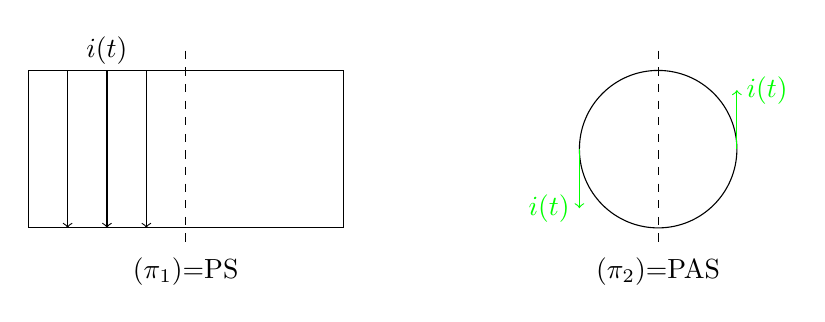
\begin{tikzpicture}[scale=1]  
                    \draw (0,0)rectangle++(4,2);
                    \draw[->] (0.5,2)--++(0,-2);
                    \draw[->] (1,2)--++(0,-2);
                    \draw[->] (1.5,2)--++(0,-2);
                    \node at (1, 2.25) {$i(t)$};
                    \draw[dashed] (2,2.25)--++(0,-2.5) node [below] {($\pi_1$)=PS};

                    \draw (8,1) circle (1);
                    \draw[dashed] (8,2.25)--++(0,-2.5) node [below] {($\pi_2$)=PAS};
                    \draw[draw=green, text=green,->] (9,1)--++(0,0.75) node [right] {$i(t)$};
                    \draw[draw=green, text=green,->] (7,1)--++(0,-0.75) node [left] {$i(t)$};
                \end{tikzpicture}
                \caption{Plans de symétrie et d'antisymétrie d'un solénoïde.}    
                \label{fig:plan_symetrie_solenoide_fini}
            \end{figure}
        \end{example}

        \begin{example}[Condensateur plan à armatures circulaire]
            Tout plan contenant l'axe est un plan de symétrie. Tout plan qui y est perpendiculaire est un plan d'antisymétrie, voir la Figure~\ref{fig:plan_symetrie_condensateur_plan_armatures_circulaire}.
            \begin{figure}
                \centering
                \tikzsetnextfilename{plan_symetrie_condensateur_plan_armatures_circulaire}
                \begin{tikzpicture}[scale=1]  
                    \draw (0,0)ellipse (2 and 0.5);
                    \draw (0,3)ellipse (2 and 0.5);
                    \node at (-1,0) {-q};
                    \node at (-1,3) {+q};
                    \draw[<->] (-2.5,0)--++(0,3) node [left, midway] {$e$};

                    \draw[draw=blue,text=blue] (0,-1.5)--++(0,5.5) node [above,shift={(0,0.25)}] {$(\pi_1$)=PS};
                    \draw[draw=blue,dashed] (0,-1.5)--++(2,1);
                    \draw[draw=blue,dashed] (0,4)--++(2,1);
                    \draw[draw=blue,dashed] (-2,1.5)--++(4,0);
                    \draw[draw=blue,dashed] (-2,1.5)--++(0.5,0.5);
                    \draw[draw=blue,dashed,text=blue] (2,1.5)--++(0.5,0.5) node [right] {($\pi_2$)=PAS};
                \end{tikzpicture}
                \caption{Plans de symétrie et d'antisymétrie d'un condensateur plan.}    
                \label{fig:plan_symetrie_condensateur_plan_armatures_circulaire}
            \end{figure} 
        \end{example}

    \subsection{Propriétés de symétrie pour le champ électromagnétique}

        Principe de Curie : si la cause (charges, courants) présente une propriété de symétrie, alors l'effet ($\vec{F}_L$) présente aussi cette propriété de symétrie. Pour le champ électromagnétique, on en déduit :
        \begin{itemize}
            \item un PS pour $\mathcal{D}$ est un PS pour $\vec{E}$ et un PAS pour $\vec{B}$;
            \item un PAS pour $\mathcal{D}$ est un PAS pour $\vec{E}$ et un PS pour $\vec{B}$.
        \end{itemize}

    \subsection[Géométrie du champ sur un PS/PAS]{Géométrie du champ électromagnétique sur un PS/PAS}

        On en déduit donc que 
        \begin{itemize}
            \item Pour un PS, on a 
            \begin{equation}
                \vec{E}(\pi(M))=\vec{E}(M)=S_{\pi}(\vec{E}(M)),
            \end{equation}
            donc $\vec{E}$ appartient au plan de symétrie en tout point du plan de symétrie. Au contraire, on a 
            \begin{equation}
                \vec{B}(\pi(M))=\vec{B}(M)=-S_{\pi}(\vec{B}(M)),
            \end{equation}
            donc $\vec{B}$ est perpendiculaire au plan de symétrie en tout point du plan de symétrie.

            \item Pour un PAS, on a 
            \begin{equation}
                \vec{E}=-S_{\pi}(\vec{E}),
            \end{equation}
            donc $\vec{E}\perp$ PAS, et
            \begin{equation}
                \vec{B}=S_{\pi}(\vec{B}),
            \end{equation}
            donc $\vec{B}\in$ PAS.
        \end{itemize}

    \subsection{Exemples}

        La méthode est la suivante :
        \begin{enumerate}
            \item Faire un choix d'un système de coordonnées adapté;
            \item Observer les invariances par translation/rotation de la distribution;
            \item Appliquer le principe de Curie : symétries et géométrie du champ.
        \end{enumerate}

        Pour un condensateur plan d'axe $(Oz)$, ou un solénoïde d'axe $(Oz)$, toute rotation autour de l'axe $(Oz)$ laisse la distribution invariante (symétrie de révolution d'axe $(Oz)$). Ainsi, la variable $\theta$ est non pertinente. De plus, tout plan contenant l'axe est un PAS. Donc $\vec{E}(r,z,t)=E(r,z,t)\vec{u_{\theta}}$ et $\vec{B}(r,z,t)=\begin{pmatrix}
                B_r(r,z,t)\\0\\B_{z}(r,z,t)
            \end{pmatrix}$.